\subsection{08.12.18}
\subsubsection{Префиксный код}
$\Lambda$ - произвольное конечное множество (алфавит). $a \in \Lambda$ - символы.\\
$\forall a \in \Lambda \; \exists l(a) \in \mathbb{N}, \exists c(a) = \{0, 1\}^{l(a)}$ - кодовая последовательность a.\\
$\forall a, b \in \Lambda, a \not= b \; c(a) \not= c(b)$. Казалось бы, это достаточное условие, чтобы по коду однозначно распознавался символ. Но рассмотрим случай:\\
$\Lambda = \{a, b\}$, $c(a) = 10$, $c(b) = 100$. Тогда последовательность $100$ получатель сообщения может начать распознавать как "a???", а поскольку 0 не является валидным кодом, получатель не сможет расшифровать сообщение без каких-то дополнительных усилий. Если же добавить в алфавит символы $d, c(d) = 01$ и $e, c(e) = 1$, сообщение $1001$ можно будет понять и как $aв$, и как $be$.\\
Чтобы избежать подобных проблем, вводят условие префиксности:\\
Код называется префиксным, если $\forall a, b \in \Lambda \; c(a) = w \Rightarrow \not\exists m \in \mathbb{N}_0: \; c(b) = w\gamma$, где $\gamma \in \{0, 1\}^m$.\\
Иначе говоря, код называется префиксным, если никакая кодовая последовательность одного символа не является началом кодовой последовательности другого символа. Заметим также, что данное условие включает в себя условие несовпадения кодов различных символов, так что в дальнейшем отдельно рассматривать мы его не будем.\\
\subsubsection{Задача об оптимальном префиксном коде}
Пусть каждому символу $a \in \Lambda$ соответствует $p(a)$ - вероятность появления этого символа в сообщении. (Поскольку сообщение состоит из одного символа, $\sum\limits_{a \in \Lambda}p(a) = 1$. Также считаем, что $\forall a \in \Lambda \; p(a) > 0$).\\
Введем ДСВ $l: \; \forall a \in \Lambda \; Pr\{l = l(a)\} = p(a)$ - длина кодовой последовательности символа в сообщении.\\
Оптимальным называется префиксный код, минимизирующий матожидание l: $E \: l = \sum\limits_{a \in \Lambda}l(a)p(a)$\\
Интуитивно понятно, что чем чаще встречается символ, тем короче должна быть его кодовая последовательность. Но вот как это формализовать?\\
Договоримся про обозначения: здесь и далее считаем, что символы с одинаковыми прибамбасами (волна, палочка, штрих, два штриха и.т.д) относятся к коду с таким же прибамбасом, обговаривать это каждый раз не будем. То есть, $C' = \{(a, l'(a), c'(a)) \; : \; a \in \Lambda\}$, например.\\
Существование оптимального префиксного кода: ну, мы знаем, что $E \: l \geq 1$, ведь в каждой кодовой последовательности должен быть хотя бы один символ. Ну и мы знаем, что в худшем случае мы можем сделать префиксный код, в котором все символы имеют одинаковые длины кодовых последовательностей и эти последовательности различны. В таком случае $\forall a \in \Lambda \; l(a) = \lceil \log_2(|\Lambda|)$, так что префиксные коды существуют и матожидание длины кодовой последовательности ограничено.\\
Лемма 1: Если в некотором (не обязательно оптимальном) коде C существует $x \in \Lambda: \; c(x) = w\alpha$, где $\alpha \in \{0, 1\}$, и при этом $\not\exists y \in \Lambda, y \not= x: \; c(y) = w\gamma$, где $\gamma \in \{0, 1\}^k$ (то есть, если w не является началом никакой другой кодовой последовательности, кроме $c(x)$), то код $C'$ такой, что $c'(x) = w, \forall y \in \Lambda, y \not= x \; c'(y) = c(y)$ во-первых будет префиксным (по построению, префиксности C и условию леммы), а во-вторых, $E \: l' = E \: l - p(x)l(x) + p(x)(l(x) - 1) = E \: l - p(x) < E \: l$.\\
Тогда получается, что код C точно не мог быть оптимальным.\\
Лемма (*), которой не было в лекции, но она удобная: если в префиксном коде C $\exists a, b \in \Lambda, a \not= b: \;p(a) < p(b), l(a) < l(b)$, то такой код не оптимален. Доказательство: проверим, что для кода $C'$, в котором $c'(a) = c(b), c'(b) = c(a), \forall x \in \Lambda, x \not= a, x \not= b \; c'(x) = c(x)$\\
$E \: l - E \: l' = p(a)l(a) + p(b)l(b) - p(a)l(b) - p(b)l(a) = p(a)(l(a) - l(b)) - p(b)(l(a) - l(b)) = (p(a) - p(b))(l(a) - l(b)) > 0$.\\
Лемма 2: Пусть $a, b \in \Lambda, a \not= b$ - два символа с наименьшими вероятностями (для определенности, $\forall x \in \Lambda \; p(x) \leq p(b) \leq p(a)$). Тогда существует оптимальный префиксный код такой, что в нем $c(a) = w0, c(b) = w1$, где $\exists k \in \mathbb{N}_0: \; w \in \{0, 1\}^k$, и это самые длинные кодовые последовательности.\\
Доказательство: пусть $C'$ - какой-то оптимальный префиксный код. По лемме (*) a и b имеют самые длинные кодовые последовательности в $C'$: $\forall x \in \Lambda, x \not= a, x \not= b \; l'(a) \geq l'(b) \geq l'(x)$. Если $c(a) = w\gamma, w \in \{0, 1\}^{l(b)}, \gamma \in \{0, 1\}^{l(a) - l(b)}$ и w не является началом никакой кодовой последовательности (а он не является, т.к. все остальные кодовые последовательности не длиннее w, и при этом никакой символ не может иметь кодовую последовательность w, так как тогда нарушалась бы префиксность $C'$), то можно сократить кодовую последовательность a, создав более оптимальный код, что противоречит оптимальности $C'$.\\
Таким образом, мы узнали, что поскольку $C'$ оптимален, $l(a) = l(b)$. Ну а теперь дело техники: пусть $c'(b) = w1$ (если заканчивается на ноль, делаем все аналогично и в конце меняем коды местами), тогда если $\exists x \in \Lambda: \; c'(x) = w0$, построим оптимальный (поскольку длины кодовых последовательностей не изменились) код С: $c(a) = c'(x), c(x) = c'(a), \forall z \in \Lambda, z \not= a, z \not= x \; c(z) = c'(z)$. Если же такого x не нашлось, то построим оптимальный (поскольку длины кодовых последовательностей не изменились) код С: $c(a) = w0, \forall z \in \Lambda, z \not= a \; c(z) = c'(z)$. Лемма доказана.\\
Лемма 3: $\forall x \in \Lambda, x \not= a, x \not= b \; p(a) \leq p(b) \leq p(x)$.\\
$\Lambda' = \Lambda \setminus \{a, b\} \cup \{\underbrace{ab}\}$, где $\underbrace{ab} \not\in \Lambda, p(\underbrace{ab}) = p(a) + p(b)$.\\
Пусть $C'$ - оптимальный префиксный код для $\Lambda'$, $c'(\underbrace{ab}) = w$. Тогда для $\Lambda$ код С:\\
$c(a) = w0, c(b) = w1, \forall x \in \Lambda, x \not= a, x \not= b \; c(x) = c'(x)$ будет оптимальным префиксным кодом.\\
Доказательство: $l(a)p(a) + l(b)p(b) = (l'(\underbrace{ab}) + 1)(p(a) + p(b)) = l'(\underbrace{ab})p(\underbrace{ab}) + p(\underbrace{ab})$ Тогда $E \: l = E \: l' + p(\underbrace{ab})$.\\
Пусть $\overline{C}$ - оптимальный код для $\Lambda$, причем $E \: \overline{l} < E \: l$.\\
По лемме 2: $\overline{c}(a) = \gamma0, \overline{c}(b) = \gamma1$.\\
Построим $\overline{C}'$ для $\Lambda'$: $\overline{c}'(\underbrace{ab}) = \gamma, \forall x \in \Lambda, x \not= a, x \not= b \; \overline{c}'(x) = \overline{c}(x)$\\
Является ли $\overline{С}'$ префиксным кодом? Да. Никакой символ по лемме (*) не мог иметь кодовую последовательность длины $> \overline{l}(a)$. Никакой символ не мог иметь кодовую последовательность w, так как $\overline{C}$ префиксный. А единственные две последовательности длины $\overline{l}(a)$, начинающиеся на w, - это коды символов a и b, которых в $\Lambda'$ нет. \\
При этом, $E \: \overline{l} = E \: \overline{l}' + p(\underbrace{ab})$. Но поскольку по предположению $E \: l = E \: l' + p(\underbrace{ab}) > E \: \overline{l} = E \: \overline{l}' + p(\underbrace{ab})$, получаем $E \: l' > E \: \overline{l}'$, что противоречит оптимальности $C'$ на $\Lambda'$.\\
Значит, предположение неверно и $E \: \overline{l} \geq E \: l$, но так как $\overline{C}$ оптимален, $E \: \overline{l} = E \: l$, то есть C оптимален. Лемма доказана.
\subsubsection{Алгоритм Хаффмана построения оптимального префиксного кода.}
Итак, нам нужно построить оптимальный префиксный код на алфавите $\Lambda$, $|\Lambda| = M$.\\
Возьмем $\Lambda_0 = \Lambda$.\\
$\forall k \in 0:(M - 3)$ возьмем $a_k, b_k \in \Lambda_k$ такие, что $\forall x \in \Lambda_k, x \not= a_k, x \not= b_k \; p_k(a_k) \leq p_k(b_k) \leq p_k(x)$ и построим $\Lambda_{k + 1} = \Lambda_{k} \setminus \{a_k, b_k\} \cup \{\underbrace{a_kb_k}\}$.\\
Для $\Lambda_{M - 2} = \{a_{M - 2}, b_{M - 2}\}$ оптимальным, очевидно, будет код $C_{M - 2}: \; c_{M - 2}(a_{M - 2}) = 0, c_{M - 2}(b_{M - 2}) = 1$, так как для него $E \: l_{M - 2} = 1$.\\
Теперь пусть для $k \in 1:(M - 2)$ у нас есть оптимальный префиксный код $C_k$ для $\Lambda_k$. По лемме 3 построим оптимальный префиксный код $C_{k - 1}$ для $\Lambda_{k - 1}$: $c_{k - 1}(a_{k - 1}) = c_k(\underbrace{a_{k - 1}b_{k - 1}})0, c_{k - 1}(b_{k - 1}) = c_k(\underbrace{a_{k - 1}b_{k - 1}})1, \forall x \in \Lambda_k, x \not= \underbrace{a_{k - 1}b_{k - 1}} \; c_{k - 1}(x) = c_k(x)$\\
Так строим, пока не получим $C_0$ - оптимальный префиксный код для $\Lambda_0 = \Lambda$.\\
Пример:\\
$\Lambda = \{a, b, c, d, e, f, g\}$, $p(a) = 0.13, p(b) = 0.08, p(c) = 0.25, p(d) = 0.18, p(e) = 0.03, p(f) = 0.12, p(g) = 0.21$\\
$a_0 = e, b_0 = b$.\\
$\Lambda_1 = \{a, \underbrace{eb}, c, d, f, g\}$, $p(a) = 0.13, p(\underbrace{eb}) = 0.11, p(c) = 0.25, p(d) = 0.18, p(f) = 0.12, p(g) = 0.21$\\
$a_1 = \underbrace{eb}, b_1 = f$
$\Lambda_2 = \{a, \underbrace{ebf}, c, d, g\}$, $p(a) = 0.13, p(\underbrace{ebf}) = 0.23, p(c) = 0.25, p(d) = 0.18, p(g) = 0.21$\\
$a_2 = a, b_2 = d$\\
$\Lambda_3 = \{\underbrace{ad}, \underbrace{ebf}, c, g\}$, $p(\underbrace{ad}) = 0.31, p(\underbrace{ebf}) = 0.23, p(c) = 0.25, p(g) = 0.21$\\
$a_3 = g, b_3 = \underbrace{ebf}$\\
$\Lambda_4 = \{\underbrace{ad}, \underbrace{gebf}, c\}$, $p(\underbrace{ad}) = 0.31, p(\underbrace{gebf}) = 0.44, p(c) = 0.25$\\
$a_4 = c, b_4 = p(\underbrace{ad})$\\
$\Lambda_5 = \{\underbrace{cad}, \underbrace{gebf}\}$, $p(\underbrace{cad}) = 0.56, p(\underbrace{gebf}) = 0.44$\\
Тогда $c_5(\underbrace{gebf}) = 0, c_5(\underbrace{cad}) = 1$. Теперь раскрываем алфавит обратно:\\
$c_4(\underbrace{gebf}) = 0, c_4(c) = 10, c_4(\underbrace{ad}) = 11$\\
$c_3(g) = 00, c_3(\underbrace{ebf}) = 01, c_3(c) = 10, c_3(\underbrace{ad}) = 11$\\
$c_2(g) = 00, c_2(\underbrace{ebf}) = 01, c_2(c) = 10, c_2(a) = 110, c_2(d) = 111$\\
$c_1(g) = 00, c_1(\underbrace{eb}) = 010, c_1(f) = 011, c_1(c) = 10, c_1(a) = 110, c_1(d) = 111$\\
$c_0(g) = 00, c_0(e) = 0100, c_0(b) = 0101, c_0(f) = 011, c_0(c) = 10, c_0(a) = 110, c_0(d) = 111$\\
$E \: l_0 = 2 * 0.21 + 4 * 0.03 + 4 * 0.08 + 3 * 0.12 + 2 * 0.25 + 3 * 0.13 + 3 * 0.18 = 2.65$\\
Заметим также, что параллельно с построением кода можно строить соответствующее ему двоичное дерево. Тогда код - это набор путей из корня в произвольную вершину в произвольном двоичном дереве, префиксный код - набор путей из корня в листья в произвольном двоичном дереве.
\begin{figure}[H]
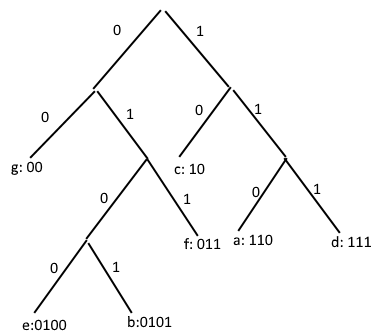
\includegraphics[width=\linewidth]{Huffman.png}
\caption{Иллюстрация к примеру.}
\label{fig:Huffman}
\end{figure}